\begin{frame}{Modos de Operación}
  \begin{columns}
    \begin{column}{0.5\textwidth}
      \only<1>{
        Sensibilidad exponencial: $\Delta d = 1$ \AA \ altera $I$ en
      un factor de $\sim 10$.

      \vspace{0.5cm}

      \begin{enumerate}
        \item \textbf{Modo de Corriente Constante:} Un lazo de
        retroalimentación ajusta la altura de la punta ($z$) para mantener
        la corriente ($I$) constante. La topografía se mapea mediante los
        voltajes del piezoeléctrico en $z$.
      \end{enumerate}
      }

      \only<2>{
      \begin{enumerate}
        \setcounter{enumi}{1}
        \item \textbf{Modo de Altura Constante:} La punta se desplaza en
        un plano ($x,y$) fijo. La topografía se deduce de las variaciones de
        corriente. Permite escaneos rápidos en superficies planas.
      \end{enumerate}
    }
    \end{column}

    \begin{column}{0.5\textwidth}
      \centering
      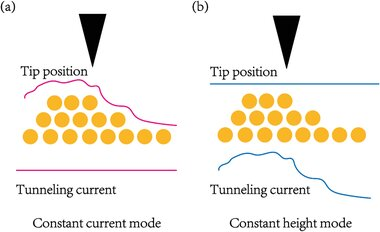
\includegraphics[width=0.95\textwidth]{images/modos de operacion stm.jpg}

      \vspace{0.2cm}
      \tiny
      \textit{Figura 1: Modos de operación del STM: (a) corriente constante
      y (b) altura constante.
      Fuente: \url{https://en.wikipedia.org/wiki/File:STM_schematic.svg}}
    \end{column}
  \end{columns}
\end{frame}

\section*{Partes del Instrumento}

\begin{frame}{Componentes Principales del STM}
  \begin{columns}
    \begin{column}{0.58\textwidth}
      \only<1>{
        \begin{itemize}
          \item \textbf{La Punta:} El ``sensor'' del equipo. Generalmente
            fabricada de un hilo de Wolframio ($\ce{W}$) o una aleación de Platino-Iridio
            ($\ce{Pt-Ir}$). Idealmente, debe terminar en un único átomo.
          \item \textbf{Escáner Piezoeléctrico:} Materiales cerámicos (como el
            PZT) que se deforman con precisión sub-angstrom al aplicarles voltaje.
            Controlan el movimiento tridimensional ($x, y, z$) de la punta.
        \end{itemize}
      }
      \only<2>{
        \begin{itemize}
          \item \textbf{Lazo de Retroalimentación (Feedback):} Electrónica
            analógica/digital que compara la corriente de tunelaje leída con un
            valor de referencia (setpoint) y corrige el voltaje del piezoeléctrico
            en el eje $z$.
        \end{itemize}
      }
    \end{column}
    \begin{column}{0.42\textwidth}
      \centering
      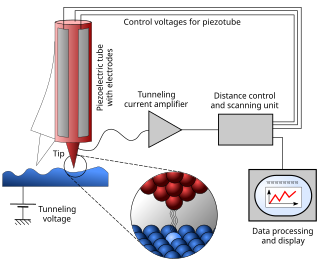
\includegraphics[width=0.9\textwidth]{images/esquema stm.png}\\
      \vspace{0.2cm}
      \tiny{\textit{Figura 2: Esquema del lazo de retroalimentación,
          amplificador de corriente de tunelaje y tubo piezoeléctrico de un STM.
          Fuente:
      \url{https://www.researchgate.net/publication/353641819_Recent_Progress_on_the_Scanning_Tunneling_Microscopy_and_Spectroscopy_Study_of_Semiconductor_Heterojunctions/figures?lo=1}}}
    \end{column}
  \end{columns}
\end{frame}

\begin{frame}{Sistemas de Aislamiento}
  Cualquier perturbación externa puede arruinar la medición a escala atómica. El
  instrumento requiere:
  \vspace{0.3cm}
  \begin{itemize}
    \item \textbf{Aislamiento de Vibraciones Mecánicas:} Se utilizan mesas
      ópticas neumáticas, sistemas de suspensión por resortes elásticos y
      amortiguación por corrientes de Foucault (Eddy currents) usando imanes y
      placas de cobre.
    \item \textbf{Aislamiento Acústico y Eléctrico:} Cámaras insonorizadas y
      blindaje electromagnético (Jaula de Faraday) para evitar ruido en la
      electrónica sensible, ya que las corrientes medidas están en el rango de
      los nanoamperios ($10^{-9}$ A).
  \end{itemize}
\end{frame}

\section*{Preparación y Colocación de la Muestra}

\begin{frame}{Requisitos y Preparación}
  \textbf{Condición Fundamental:}\\
  La muestra debe ser conductora o semiconductora. El STM no funciona con
  aislantes puros (para ello se usaría AFM).
  \begin{columns}
    \begin{column}{0.6\textwidth}
      \textbf{Protocolos de Preparación:}
      \only<1>{
        \begin{itemize}
          \item \textbf{Exfoliación In-Situ:} Materiales en capas (como HOPG -
            Grafito Pirolítico Altamente Orientado) se exfolian con cinta adhesiva
            para revelar una superficie atómicamente plana justo antes de medir.
        \end{itemize}
      }
      \only<2>{
        \begin{itemize}
          \item \textbf{Bombardeo Iónico y Recocido:} Para metales y
            semiconductores. Se bombardean con iones de Argón para quitar óxidos e
            impurezas, y luego se calientan (recocido) para reconstruir la
            estructura cristalina superficial.
        \end{itemize}
      }
    \end{column}
    \begin{column}{0.4\textwidth}
      \centering
      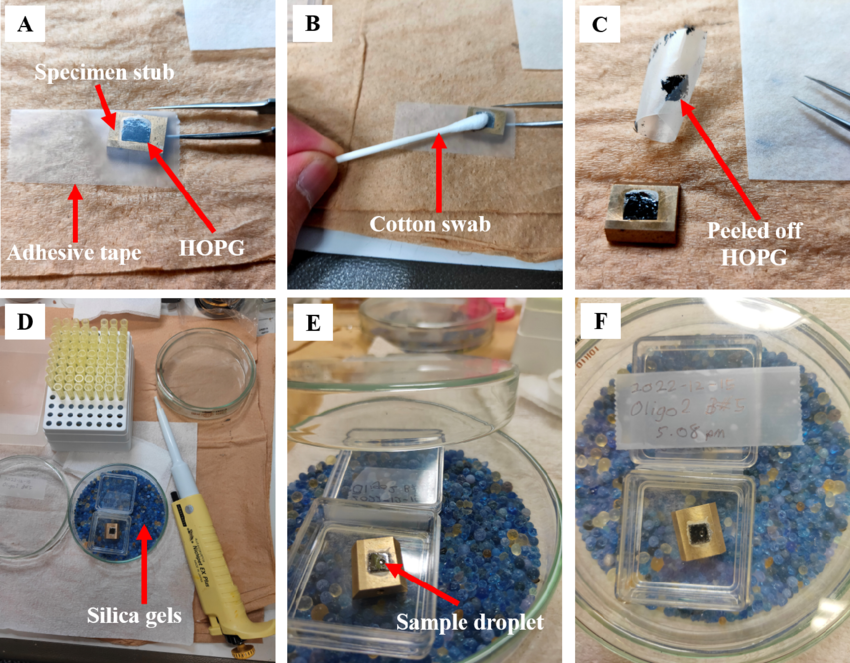
\includegraphics[width=0.8\textwidth]{images/preparacion muestra stm.png}\\
      \vspace{0.2cm}
      \tiny{\textit{Figura 3: Proceso de preparación de la muestra mediante la
          técnica de exfoliación (cleaving) de grafito pirolítico altamente
          orientado (HOPG). Fuente:
      \url{https://www.researchgate.net/publication/395101014_Exploring_the_Involvement_of_PINK1_in_Parkinson\%27s_Disease_A_Scanning_Tunnelling_Microscopy_Study_of_Electron_Transfer_in_Synthetic_DNA_Samples/figures?lo=1}}}
    \end{column}
  \end{columns}
\end{frame}

\begin{frame}{Condiciones de Vacío y Transferencia}
  \begin{columns}
    \begin{column}{0.58\textwidth}
      \only<1>{
        \begin{itemize}
          \item \textbf{Ultra Alto Vacío (UHV):} Para que la superficie preparada
            no se contamine casi instantáneamente con moléculas del aire, el
            instrumento debe estar contenido en cámaras UHV (presiones del orden
            de $10^{-10}$ Torr).
          \item \textbf{Montaje en el Portamuestras:} La muestra se fija a placas
            metálicas especiales (frecuentemente de Molibdeno o Tántalo por su
            resistencia térmica) usando soldadura por puntos o clips metálicos,
            garantizando contacto eléctrico.
        \end{itemize}
      }
      \only<2>{
        \begin{itemize}
          \item \textbf{Transferencia:} El portamuestras se inserta en el
            microscopio mediante manipuladores magnéticos, llamados ``brazos de
            transferencia'', sin romper el vacío de la cámara principal.
        \end{itemize}
      }
    \end{column}
    \begin{column}{0.42\textwidth}
      \centering
      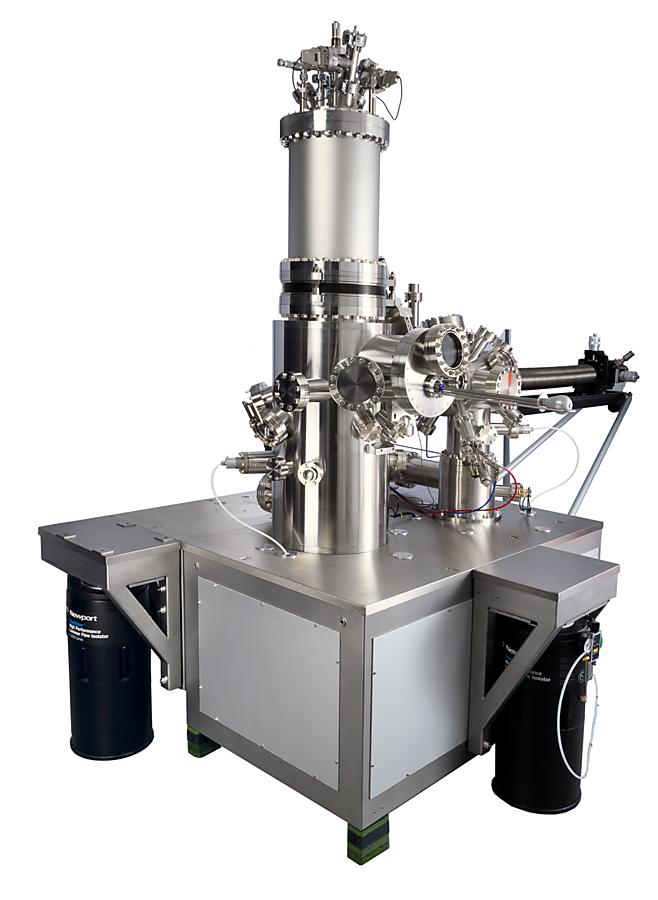
\includegraphics[width=0.6\textwidth]{images/stm.jpg}\\
      \vspace{0.2cm}
      \tiny{\textit{Figura 4: Sistema de ultra alto vacío (UHV) para microscopía
          de efecto túnel, equipado con cámara principal y manipuladores para la
          transferencia de muestras. Fuente:
      \url{https://scientaomicron.com/en/products-solutions/SPM/LT-STM-Lab}}}
    \end{column}
  \end{columns}
\end{frame}
